\documentclass{oblivoir}

\usepackage{amsthm}
\usepackage{thmtools}

\usepackage{url}

%\usepackage{ansform}
\usepackage{ikps}

\usepackage{graphicx}
%https://www.overleaf.com/learn/latex/Inserting_Images

\usepackage{listings}
\usepackage{xcolor}
\declaretheoremstyle[% spaceabove=6pt,spacebelow=6pt, headfont=\color{MainColorOne}\sffamily\bfseries, notefont=\mdseries, notebraces={[}{]}, bodyfont=\normalfont,
headpunct={},
postheadspace=1em,
%qed=▣,
]{maintheorem}

\declaretheorem[%
name=정의,
style=maintheorem,
numberwithin=section, shaded={%bgcolor=MainColorThree!20,
margin=.5em}]{dfn}
% \begin{dfn}[]
% \end{dfn}

\newtheorem{theorem}{Theorem}[section]
\newtheorem{corollary}{Corollary}[theorem]
\newtheorem{lemma}[theorem]{Lemma}
%https://www.overleaf.com/learn/latex/Theorems_and_proofs

\definecolor{mGreen}{rgb}{0,0.6,0}
\definecolor{mGray}{rgb}{0.5,0.5,0.5}
\definecolor{mPurple}{rgb}{0.58,0,0.82}
\definecolor{backgroundColour}{rgb}{0.95,0.95,0.92}
%https://tex.stackexchange.com/questions/348651/c-code-to-add-in-the-document
\lstdefinestyle{CStyle}{
    backgroundcolor=\color{backgroundColour},   
    commentstyle=\color{mGreen},
    keywordstyle=\color{magenta},
    numberstyle=\tiny\color{mGray},
    stringstyle=\color{mPurple},
    basicstyle=\footnotesize,
    breakatwhitespace=false,         
    breaklines=true,                 
    captionpos=b,                    
    keepspaces=true,                 
    numbers=left,                    
    numbersep=5pt,                  
    showspaces=false,                
    showstringspaces=false,
    showtabs=false,                  
    tabsize=2,
    language=C
}

\title{Introduction to Quick Sort}
\author{EUnS}


%https://tex.stackexchange.com/questions/246/when-should-i-use-input-vs-include
\begin{document}
    

\maketitle


\tableofcontents



\section{소개}

\begin{itemize}
    \item 일반적으로 가장 많이 사용하는 정렬 알고리즘
    \item 비교 정렬
    \item 내부정렬
    \item 불안정 정렬
    \item 평균 복잡도: $O(n \lg n)$
    \item 최악의 복잡도 : $O(n^2)$
    \item C++ std::sort의 내부구현이 퀵소트로 되어있음\footnote{정확하게는 introsort : quicksort와 heapsort, insertionsort를 셋 다 사용한다.}
\end{itemize}

\section{의사코드 및 동작}

분할 정복(divide and conquer) 방법을 통해 설계 되었다.
작동의 이해는 당장에 유튜브에 검색만해봐도 동작 설명하는 5분짜리 유튜브가 많으니 그걸 참고하는게 편하다.

\begin{lstlisting}[style = CStyle]    
QUICKSORT(A,p,r)
    if p < r
        q = PARTITION(A,p,r)
        QUICKSORT(A,p,q-1)
        QUICKSORT(A,q+1,r)
\end{lstlisting}

\textbf{Lomuto’s Partition Scheme}
\begin{lstlisting}[style = CStyle]
PARTITION(A ,p ,r)
    x= A[r] //pivot
    i = p-1
    for j = p to r-1
        if A[j]<= x
            i = i + 1
            exchange A[i] with A[j]
    exchange A[i+1] with A[r]
    return i + 1
\end{lstlisting}

Hoare, C. A. R.이 1961년 처음으로 Quick sort를 제안했다. PARTITION은 현재 일반적으로 Lomuto가 제안(1999)한 PARTITION이 유명하여 이를 기준으로 설명하며, Hoare가 제안한 Partition의 두 프로시저의 비교는 후에 따로 다룬다.


PARTITION 프로시저의 시간복잡도는 $\Theta(n)$이다.

\begin{figure}[h!]
    \centering
    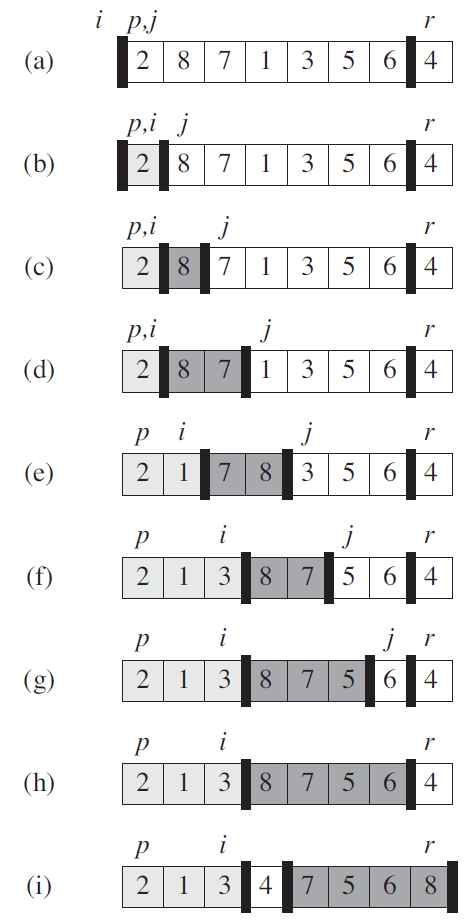
\includegraphics[scale=0.7]{pic/q1.png}
    \caption{quick sort 작동 예시\cite{reference1}}
\end{figure}


%
%성능 참고 : \href{https://www.acmicpc.net/blog/view/58}{정렬 알고리즘 비교}
%정렬 알고리즘 비교
% https://en.wikibooks.org/wiki/LaTeX/Hyperlinks#\hyperref
\newpage



\section{여러 기초 지식}

\subsection{시간복잡도}

\begin{dfn}[복잡도]
    상한, 하한,  
    \begin{itemize}

        \item 상한 big O $O$
        
        함수 $f(n), g(n)$에 대해서 $0 \le f(n) \le cg(n) ( \forall n \leq n_0)$을 만족하는 $n_0$, 양의 상수 $c$가 존재할때 $f(n) = O(g(n))$이라한다.
        
        \item 하한 omega $\Omega$

        함수 $f(n), g(n)$에 대해서 $0 \le cg(n) \le f(n) ( \forall n \leq n_0)$을 만족하는 $n_0$, 양의 상수 $c$가 존재할때 $f(n) = \Omega(g(n))$이라한다.

        \item Theta $\Theta$

        $\Theta(g(n))$일 필요충분 조건은 $f(n) = O(g(n))$이고 $f(n) = \Omega(g(n))$이 성립할때 이다.
    \end{itemize}
\end{dfn}

\subsection{조화 급수의 상한과 하한}



$\sum_{k=1}^{n} \dfrac{1}{k} = \Theta(\lg n)$

감소 함수 $f(k)$에 대해서 다음이 성립한다

$$\int_{m-1}^{n}f(x)dx \le \sum_{k=m}^n f(k) \le \int_{m}^{n+1}f(x)dx$$


\begin{figure}[h!]
    \centering
    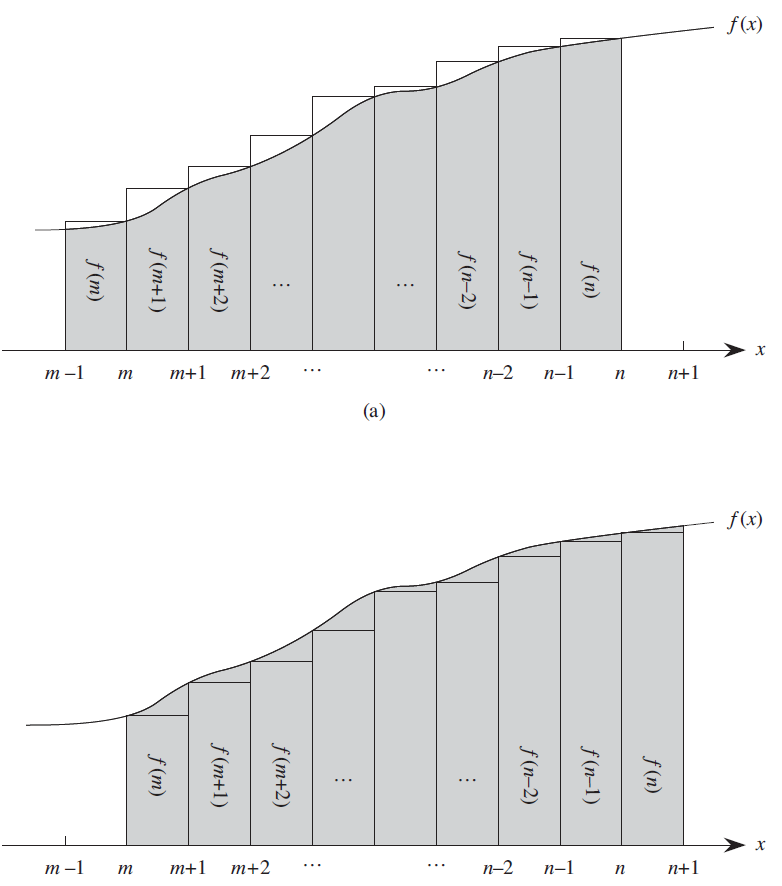
\includegraphics[scale=0.5]{./QuickSort/pic/q5.png}
    \caption{증가함수의 대소비교\cite{reference1}}
\end{figure}

증가함수 $f(k)$에 대해 다음이 성립함을 그림 4를 통해서 이해 할 수있다. 감소함수는 이와 반대로 생각하면 쉽게 해당 부등식을 이해할 수 있다.

$$\int_{m}^{n+1}f(x)dx \le \sum_{k=m}^n f(k) \le \int_{m-1}^{n}f(x)dx$$

다음 두가지 방식으로 계산한다

$\sum_{k=2}^n \dfrac{1}{k}+1 \le \int_{2}^{n+1}f(x)dx +1= \ln (x)+1 = O(\ln x)$

$\int_{1}^{n+1}f(x)dx =\ln (x+1) = \Omega(\ln x) \le \sum_{k=1}^n \dfrac{1}{k} $

따라서 $\sum_{k=1}^n \dfrac{1}{k} = \Theta(\lg n)$



\subsection{확률} Indicator random variables

\begin{align*}
    I\left\{ A \right\} =  
\begin{cases}
    1 &\mbox{( $H$ 발생)} \\
    0 &\mbox{( $\bar{H}$ 발생)}
\end{cases}    
\end{align*}


\begin{align*}
    E[X_A] &=  E[I \left\{ A \right\} ] \\
    &= 1 \times \Pr (A) + 0 \times \Pr(\bar{A}) \text{\footnotemark} \\
    &=\Pr (A)     
\end{align*}
\footnotetext{Pr은 A가 일어날 확률이다}
% https://tex.stackexchange.com/questions/21813/footnote-in-math-mode




\section{대략적인 복잡도 분석}


해당절과 다음절의 복잡도 분석은 quicksort에 모든 입력값에 중복값이 존재 하지않음을 미리 가정하고있다.

\subsection{최악의 분할 케이스} 

최악의 경우 분할 케이스를 생각해보자 
이는 왼쪽 오른쪽 분할이 한쪽으로 쏠려(오름차순,내림차순) 극도로 불균형하게 일어났을때이다.
피봇값에 의한 분할이 아예 일어나지 않을 때 최악의 케이스가 된다.
이때 비용을 나타낸 재귀함수다.
$$T(n) = T(n-1) + cn $$
\begin{align*}
    T(n) &= T(n-1) + cn \\
    &= T(n-2) + c(n-1) +cn \\
    &= c\sum^{n}_{k=1}k \\
    &= \dfrac{1}{2} cn^{2}\\
    &= \Theta (n^{2})    
\end{align*}


따라서 시간복잡도는 $\Theta(n^2)$이다.

\subsection{최선의 분할 케이스} 

정확하게 반으로 나누어 졌을때 최선의 분할 케이스이다.

이때의 비용을 나타낸 재귀함수는
$$T(n) = 2T(\dfrac{n}{2}) + cn$$
이다.

\begin{figure}[h!]
    \centering
    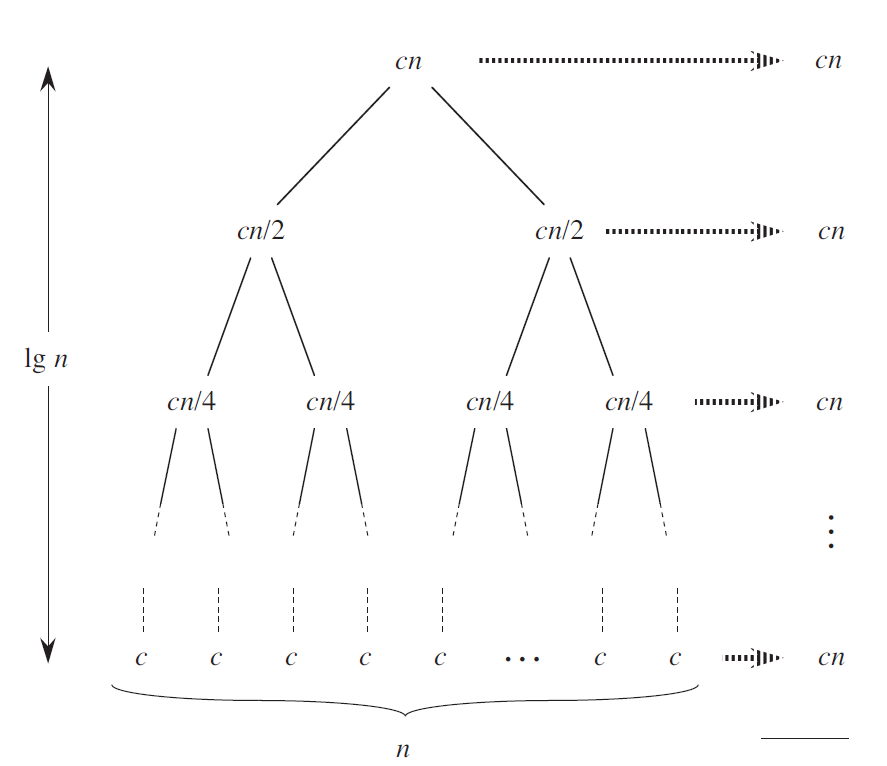
\includegraphics[scale=0.5]{./QuickSort/pic/q2.png}
    \caption{quick sort 최선의 분할 케이스 재귀 트리\cite{reference1}}
\end{figure}
그림 2의 재귀트리를 통해서 전체 비용을 계산하여 시간복잡도를 구하면 $\Theta(n \lg n)$이다. \footnote{marster theory를 사용하여 바로 구해도 된다.}

\subsection{일반적인 케이스 직관적인 방법} 
평균적인 경우로 생각해볼수있는 다음 두가지 경우에 대해서 논의를 해 볼 것이다.
\begin{itemize}
    \item 항상 9:1로 분할하는 경우
    \item 최악의 경우와 최선의 경우가 번갈아 나타나는 경우
\end{itemize}

\subsubsection{항상 9:1로 분할하는 경우}

\begin{figure}[h!]
    %\centering
    \raggedleft
    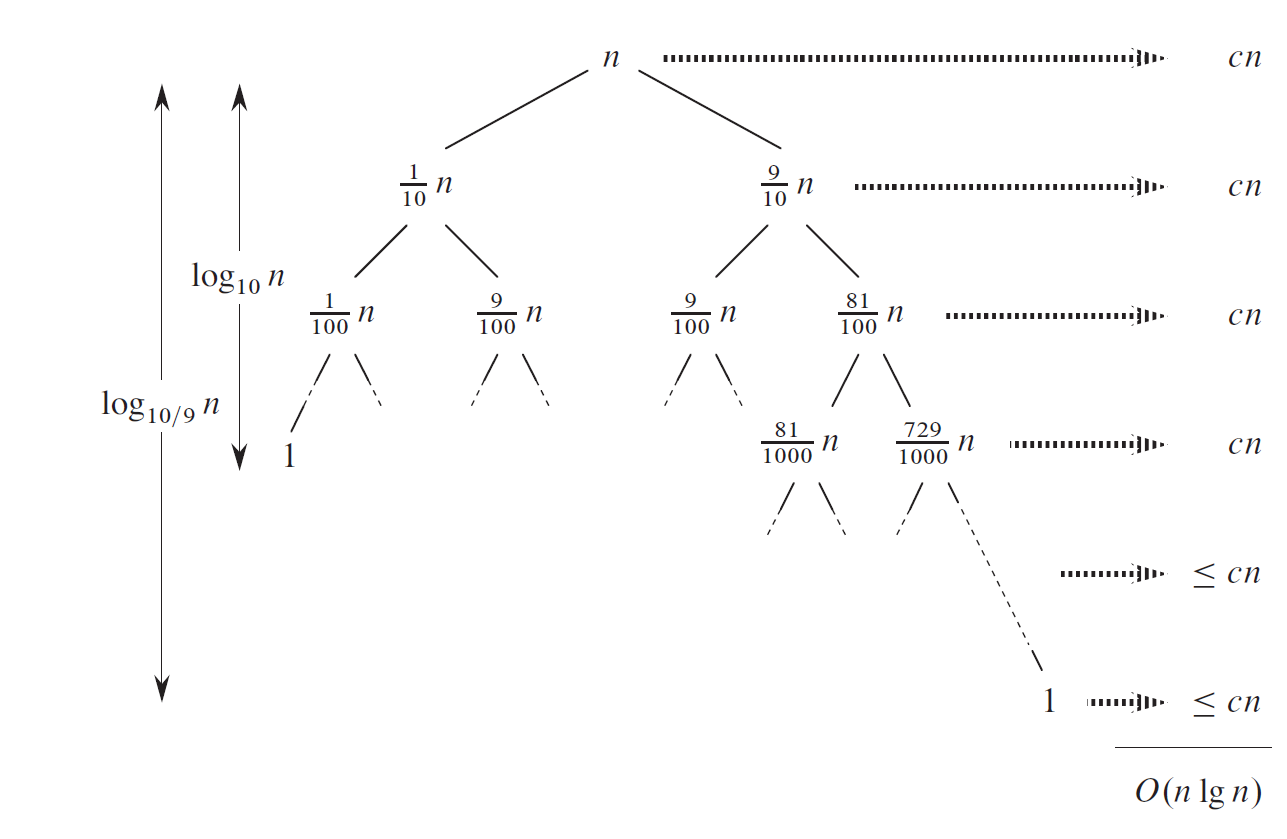
\includegraphics[scale=0.4]{./QuickSort/pic/q9.png}
    \caption{9:1로 분할하는 재귀 트리\cite{reference1}}
\end{figure}
다음의 경우 재귀 함수는 다음이 성립한다.
$$T(n) \le T\left(\dfrac{9n}{10}\right) + T\left(\dfrac{n}{10}\right)+ cn$$


이다. 
이때 재귀트리는 깊이 $\log_{10}n$까지 각 깊이의 비용이 $cn$이고 그 밑 부터는 $cn$보다 작은 비용이 든다 따라서 깊이 $\log_{10/9}n$에 각 깊이 비용 $cn$인것보다 비용이 작으므로 $n\log_{10/9}n = O(n \log n)$이 된다. 따라서 $T(n) = \Theta(n \log n)$


\subsubsection{최악의 경우와 최선의 경우가 번갈아 나타나는 경우}

\begin{figure}[h!]
    \centering
    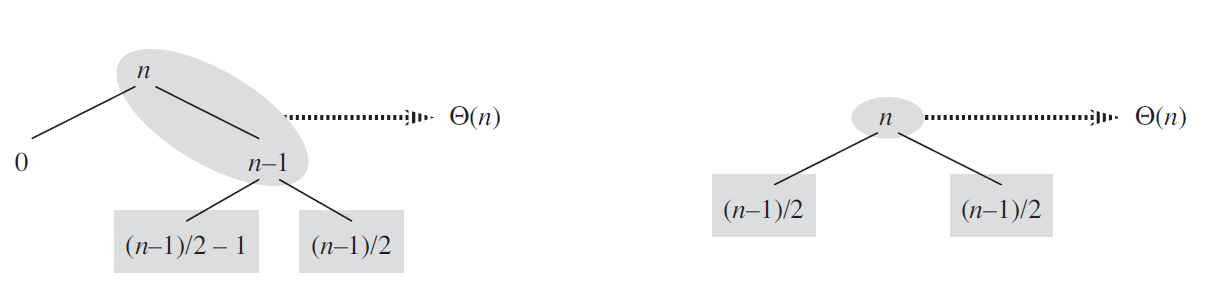
\includegraphics[scale=0.5]{./QuickSort/pic/q3.png}
    \caption{최악,최선이 번갈아 나타나는 재귀 트리\cite{reference1}}
\end{figure}

T(n) 일때의 시간복잡도와 T(n-1)일때의 시간복잡도는 둘다 $\Theta(n)$이다. 따라서 이 둘의 시간복잡도를 합쳐도 결국 $\Theta(n)$이고 이를 합쳐서 보면 결국에 최선의 분할 케이스가 된다 따라서 이때의 시간복잡도는 결국 $\Theta(n \lg n)$이다.



\section{상세 분석}

\subsection{최악의 케이스 분석 }


실제 재귀함수를 일반화 식은 다음이 된다.

$$T(n) = \max_{0 \le q \le n-1}(T(q) + T(n-q-1)) + \Theta(n)$$

이때 $T(n)$이 $\Theta(n^2)$임을 보이면된다.
치환법을 이용해서 이 점화식을 풀수있다.
$T(n) \le c_1n^2$이라 가정하자. 그러면

$$T(n) \le \max_{0 \le q \le n-1}(c_1q^2 + c_1(n-q-1)^2) + \Theta(n)$$

이 성립한다. 

$0 \le q \le n-1$인 $c_1q^2 + c_1(n-q-1)^2$에 대해서 

$f(q) = c_1q^2 + c_1(n-q-1)^2$ 이라하고 $f'(q) = 2c_1q - 2c_1(n-q-1)$이므로 $q=\dfrac{n-1}{2}$일때 극솟값을 가진다. 이 극솟값은 $q$의 존재 범위에 포함되고 따라서 이차함수의 특성에 따라 양 끝점이 최댓값이 될수있는 후보가된다. $q=0$일때와 $q=n-1$일때 극댓값을 가지는데 이때의 두 함숫값은 같아서 둘중 어느값을 택해도 최댓값이 된다.

\begin{align*}
    T(n) & \le c_1(n-1)^2 + \Theta(n) \\
    & \le c_1n^2 - c(2n-1) + \Theta(n) \\
    & \le c_1n^2    
\end{align*}


이때 $\Theta(n) = dn$에서 $ c_1 > d $인 상수 $c_1$을 가지게 함으로 써 결과적으로 $T(n)$이 $c_1n^2$보다 작거나 같음을 보일수있다. 반대로 $c_2n^2 \le T(n)$임을 가정하고  $ c_2 < d $인 상수를 잡음으로 $T(n)$이 $c_2n^2$보다 크거나 같음을 보일수있다. 따라서 $T(n) = \Theta(n^2)$를 얻을 수 있다.


\subsection{기대 수행 시간}

1 부터 모든 n에 대해서 모든 비용의 평균.

%$\dfrac{\sum_{i=1}^{n}E[X_i]}{n}$

\begin{align*}
    E[X] &= E\left[ \sum_{i=1}^{n}X_i \right] \\
    &= \sum_{i=1}^{n}E\left[X_i \right]   
\end{align*}
 
시간복잡도를 분석하기위해서 다음의 보조정리를 이용한다.


% Let X be the number of comparisons performed in line 4 of PARTITION over the entire execution of QUICKSORT on an n-element array. 

% Then the running time of QUICKSORT is O(n + X)
\begin{lemma}
    X가 길이가 n인 배열에서 QUICKSORT의 전체 실행에 대해서 PARTITION의 4행에서 수행된 비교문의 실행 수라고 가정하면 QUICKSORT의 실행시간은 O(N+X)이다.    
\end{lemma}


% By the discussion above, the algorithm makes at most n calls to PARTITION, each of which does a constant amount of work and then executes the for loop some number of times. 
% Each iteration of the for loop executes line 4.

%  PARTITION에 대한 모든 호출에서 수행 된 비교의 총 수인 X를 계산하는 것이다.

% PARTITION에 대한 각 호출에서 얼마나 많은 비교가 이루어 졌는지 분석하려고 시도하지 않습니다.

%  오히려 총 비교 수에 대한 전반적인 경계를 유도합니다.

\begin{proof}
    알고리즘은 PARTITION을 최대 n 회 호출한다. 각 호출은 for 루프를 실행하는데, for 루프의 각 반복은 4행 비교문을 실행한다.    
\end{proof}

따라서 모든 호출에 대해서 총 비교수 X를 구하는 문제로 바뀌는데 각 호출에 대한 비교를 분석하지않고 총 비교수를 계산한다.
그렇게 하기 위해 배열 $A = \{z_1 , z_2, ... , z_n\}$의 각 요소가 내림차순으로 정렬되어있다고 생각한다. 또한 집합 $Z_{ij} = \{z_i, z_{i+1}, ..., z_j\}$라 정의한다. 여기서 $z_i$와 $z_j$는 최대 한번 비교된다. 이유는 PARTITION에서 비교를 하는 경우는 하나의 원소가 pivot으로 선택 되었을 때인데, 이후에 이 pivot은 절대로 다른 원소와 비교하지 않는다.
따라서
%indicator random variables
$X_{ij} = I\{ z_i$가 $z_j$와 비교한다 $\}$

$ X = \sum_{i=1}^{n-1}\sum_{j=i+1}^{n} X_{ij}$

\begin{align*}
    E[x] &= E \left[ \sum_{i=1}^{n-1}\sum_{j=i+1}^{n} X_{ij} \right] \\
    &= \sum_{i=1}^{n-1}\sum_{j=i+1}^{n} E\left[X_{ij} \right] \\
    &= \sum_{i=1}^{n-1}\sum_{j=i+1}^{n}Pr\{ z_i \mbox{가} z_j\mbox{와 비교한다} \} 
\end{align*}    
    
\begin{align*}
    Pr\{ z_i \mbox{가} z_j\mbox{와 비교한다} 
    &= Pr\{ Z_{ij}\mbox{에서} z_i \mbox{또는} z_j\mbox{가 첫번째로 선택된다.}\}\\
    &= Pr\{ Z_{ij} \mbox{에서} z_i \mbox{가 첫번째로 선택된다}.\} + Pr\{ Z_{ij}\mbox{에서} z_j \mbox{가 첫번째로 선택된다.}\} \\
    &= \dfrac{1}{j-i+1} + \dfrac{1}{j-i+1} \\
    &= \dfrac{2}{j-i+1}    
\end{align*}
    

$$E[X] =  \sum_{i=1}^{n-1}\sum_{j=i+1}^{n} \dfrac{2}{j-i+1}$$

이는 $j-i$을 $k$로 치환해서 상한을 얻을 수 있다.

\begin{align*}
    E[X] & = \sum_{i=1}^{n-1}\sum_{j=i+1}^{n} \dfrac{2}{j-i+1}\\
    & =  \sum_{i=1}^{n-1}\sum_{k = 1}^{n-i} \dfrac{2}{k+1} \\
    & \le \sum_{i=1}^{n-1}\sum_{k = 1}^{n} \dfrac{2}{k} \\
    & \le \sum_{i=1}^{n-1} c\lg n \\
    & \le c n \lg n    
\end{align*}


$$E[X]= O(n \lg n)$$

하한은 다음과 같이 직접구한다.
\begin{align*}    
E[X] &= \sum_{i=1}^{n-1}\sum_{k = 1}^{n-i} \dfrac{2}{k+1} \\
& = \sum_{k = 1}^{n-1} \dfrac{2}{k+1} + \sum_{k = 1}^{n-2} \dfrac{2}{k+1} + \cdots + \sum_{k = 1}^{1} \dfrac{2}{k+1}\\
& = (n-1)\dfrac{2}{1+1} + (n-2)\dfrac{2}{2+1} + \cdots +1 \times \dfrac{2}{(n-1)+1}\\
& = \sum_{k=1}^{n-1} \dfrac{2}{k+1} \times (n-k)\\
& = \sum_{k=1}^{n-1} \left( \dfrac{2n}{k+1} -\dfrac{2k}{k+1}\right)\\
& = 2n \sum_{k=1}^{n-1} \dfrac{1}{k+1} - 2\sum_{k=1}^{n-1} \dfrac{k}{k+1}\\
& \ge 2nc\lg n - 2(n-1) \left(\because -\sum_{k=1}^{n-1} \dfrac{k}{k+1} \ge -\sum_{k=1}^{n-1}\left( \dfrac{k}{k+1}+\dfrac{1}{k+1}  \right)\right)\\
& \ge \Omega(n\lg n) 
\end{align*}

따라서 $$\Theta(n\lg n)$$
%%%%%%%%%%%%%%%%%%%%%%%%%%%%%%%%%%%%%%%%%%%%%
\subsection{Hoare's Partition VS Lomuto's Partition}

\textbf{Lomuto’s Partition Scheme}
\begin{lstlisting}[style = CStyle]
PARTITION(A ,p ,r)
    x= A[r] //pivot
    i = p-1
    for j = p to r-1
        if A[j]<= x
            i = i + 1
            exchange A[i] with A[j]
    exchange A[i+1] with A[r]
    return i + 1
\end{lstlisting}


\textbf{Hoare's partition scheme}

\begin{lstlisting}[style = CStyle]
PARTITION(A ,p ,r)
    x= A[r] //pivot
    i = p
    j = r
    while TRUE
        repeat
            j = j - 1
        until A[j] <= x
        repeat
            i = i + 1
        until A[i] >= x
        if i < j
            exchange  A[i] with A[j]
        else return j
\end{lstlisting}


다음 사이트의 답변을 번역했습니다 \href{https://cs.stackexchange.com/questions/11458/quicksort-partitioning-hoare-vs-lomuto}{stackexchange}\\

이해하기 편하고 간편한 알고리즘을 따질때 Lomuto’s Partition이 간편하다. 그렇기에 우리들이 알고리즘을 이렇게 기억하고 있는것일 것이다. 성능적인 측면만 따지면 다음을 비교해 볼 수 있다.

\subsubsection{비교 횟수}
모든 요소가 피봇가 비교하기 때문에 둘다 n-1번 비교한다.

\subsubsection{스왑 횟수}
Lomuto's Partition의 경우 $1 <= x <= n$인 pivot값 $x$에 대해서 스왑은 정확히 $x-1$번 수행한다.
$$\dfrac{1}{n} \sum_{x=1}^{n}(x-1) = \dfrac{n-1}{2}$$

Hoare's Partition의 경우 i는 피봇값보다 큰값 j는 피봇보다 작은 값에 대해서 스왑을 실행한다. 이 스왑을 수행하는 i의 수와 j의 수는 언제나 같은데 (당연히 쌍으로 교환하니까) 이 쌍의 수는 결과적으로  초기하 분포\footnote{학교에서 통계학을 안들어서 저도 잘 모릅니다 ㅠㅠ}를 따른다 따라서 
쌍수는 $\dfrac{(n-x)(x-1)}{n-1}$이 된다.

$$\dfrac{1}{n} \sum_{x=1}^{n} \dfrac{(n-x)(x-1)}{n-1} = \dfrac{n-2}{6}$$



\subsubsection{정렬이 이미 되어있는경우}
Hoare's Partition은 스왑을 실행하지않는다 그러나 Lomuto’s Partition은 $n/2$만큼의 스왑을 수행한다.

\subsubsection{모든 배열이 같은 값으로 설정 되어있을때}

Hoare's Partition는 무한루프에 빠진다. Lomuto’s Partition인 경우 모든 단일 요소에 대해서 스왑을 실행하며 i = n 이 되어 최악의 파티션 또한 가지게되어 수행시간은 $\Theta(n^2)$이 된다.

Hoare's Partition은 실질적인 측면에서볼때 활용도가 \textbf{매우매우매우매우매우매우매우매우매우} 떨어진다. 버그를 내기 매우 쉬운 알고리즘이고 코드 가독성 또한 매우 떨어진다 또한 결정적으로 중복값의 처리가 안되며 이를 고칠시에 결국 성능이 Lomuto’s Partition보다 느리게 된다.\footnote{
참고 : \href{https://stackoverflow.com/questions/7198121/quicksort-and-hoare-partition}{hoare}}

다음의 실제 테스트 결과를 봐도 알 수 있다.\footnote{사진의 출처인데
\href{http://rohitja.in/lomuto-hoare-partitioning.html}{Hoare, Lomuto testing} 테스트 케이스가 상당히 아쉬움을 알 수 있다.}

\begin{figure}[h!]
    \centering
    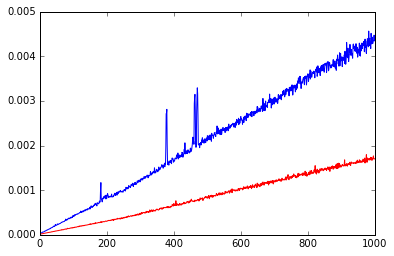
\includegraphics[scale=0.8]{{pic/q7.png}}
    %\caption{}
\end{figure}



%%%%%%%%%%%%%%%%%%%%%%%%%%%%%%%%%%%%%%%%%%%%%
\section{Quick sort의 캐시 히트율}

\begin{figure}[h!]
    \centering
    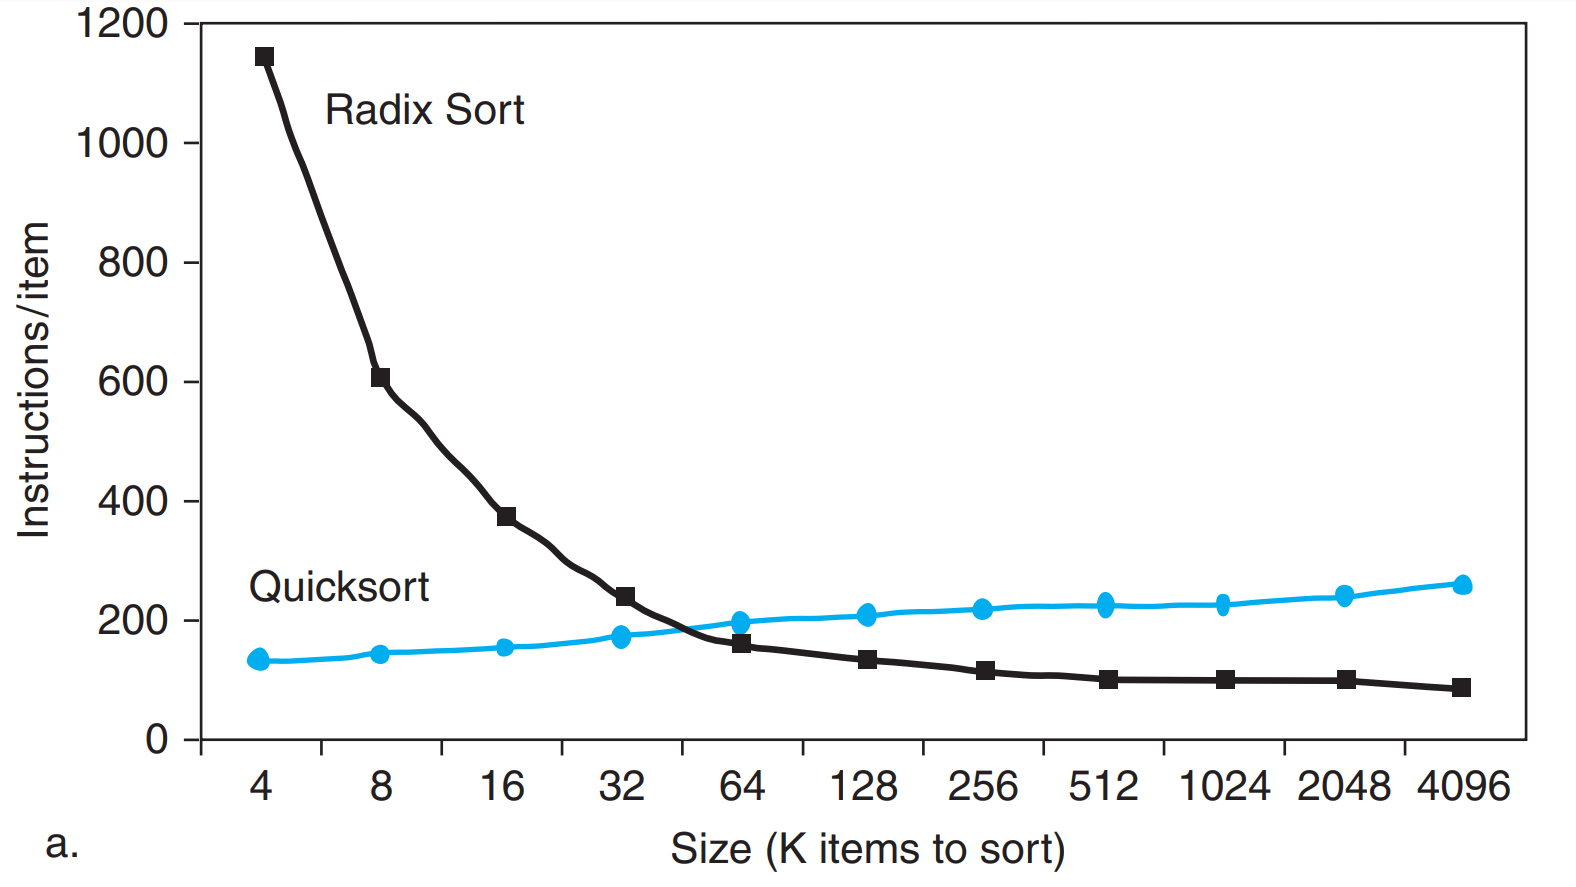
\includegraphics[scale=0.3]{{pic/quick1.png}}
\end{figure}

다음은 Radix sort(기수 정렬)과 Quick sort의 입력 n에 따른 수행 명령어 수/n를 나타낸 것이다. 
기수 정렬의 시간복잡도는 $O(n)$이나 최고차항의 계수가 커서 초반 입력 n에 대해서는 Quick sort가 빠른 것을 보여준다.

그러나 실제 수행시간과 캐시 미스율를 비교해 봤을때, 퀵소트가 높은 캐시 적중률로인해 기수정렬보다 약간 더 빠름을 볼 수 있다.
이는 알고리즘적인 부분만으로는 알수없는 결과기에 실제 컴퓨터 구조의 캐시 개념을 알아야한다.
작성자 의견: 해당 그래프에서 n의 수치가 최대가 5000으로 나와있는걸 생각해볼때 값이 정말 커지면 결국에는 시간복잡도에 따라 기수정렬이 더 빠름이 명확할것으로 예상한다.


\newpage

\begin{figure}[h!]
    \centering
    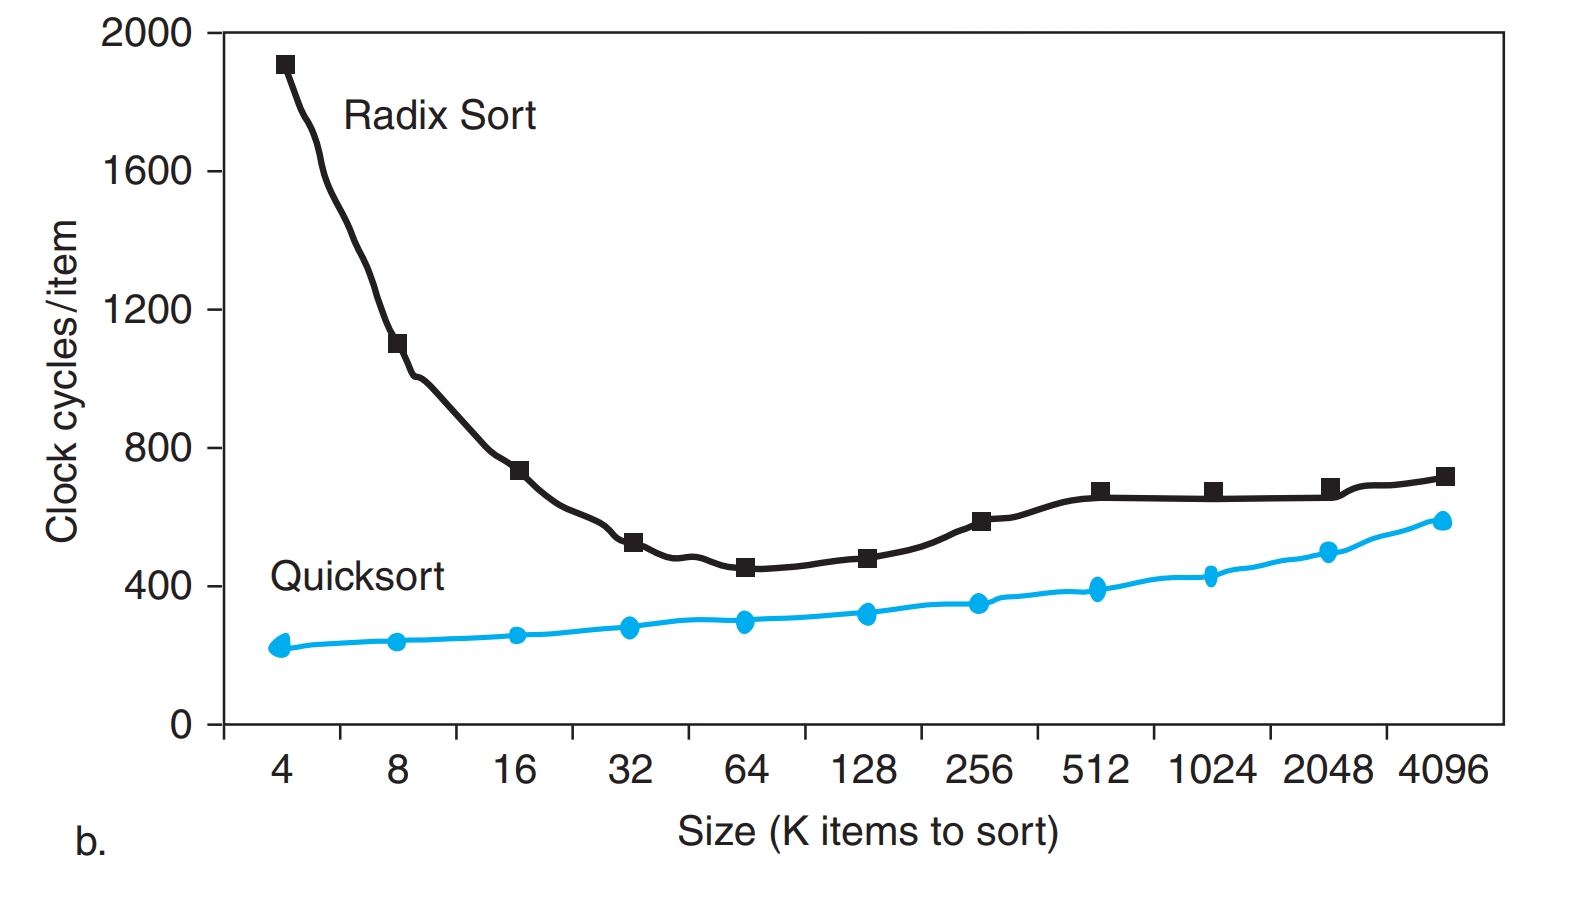
\includegraphics[scale=0.3]{{pic/quick2.png}}
    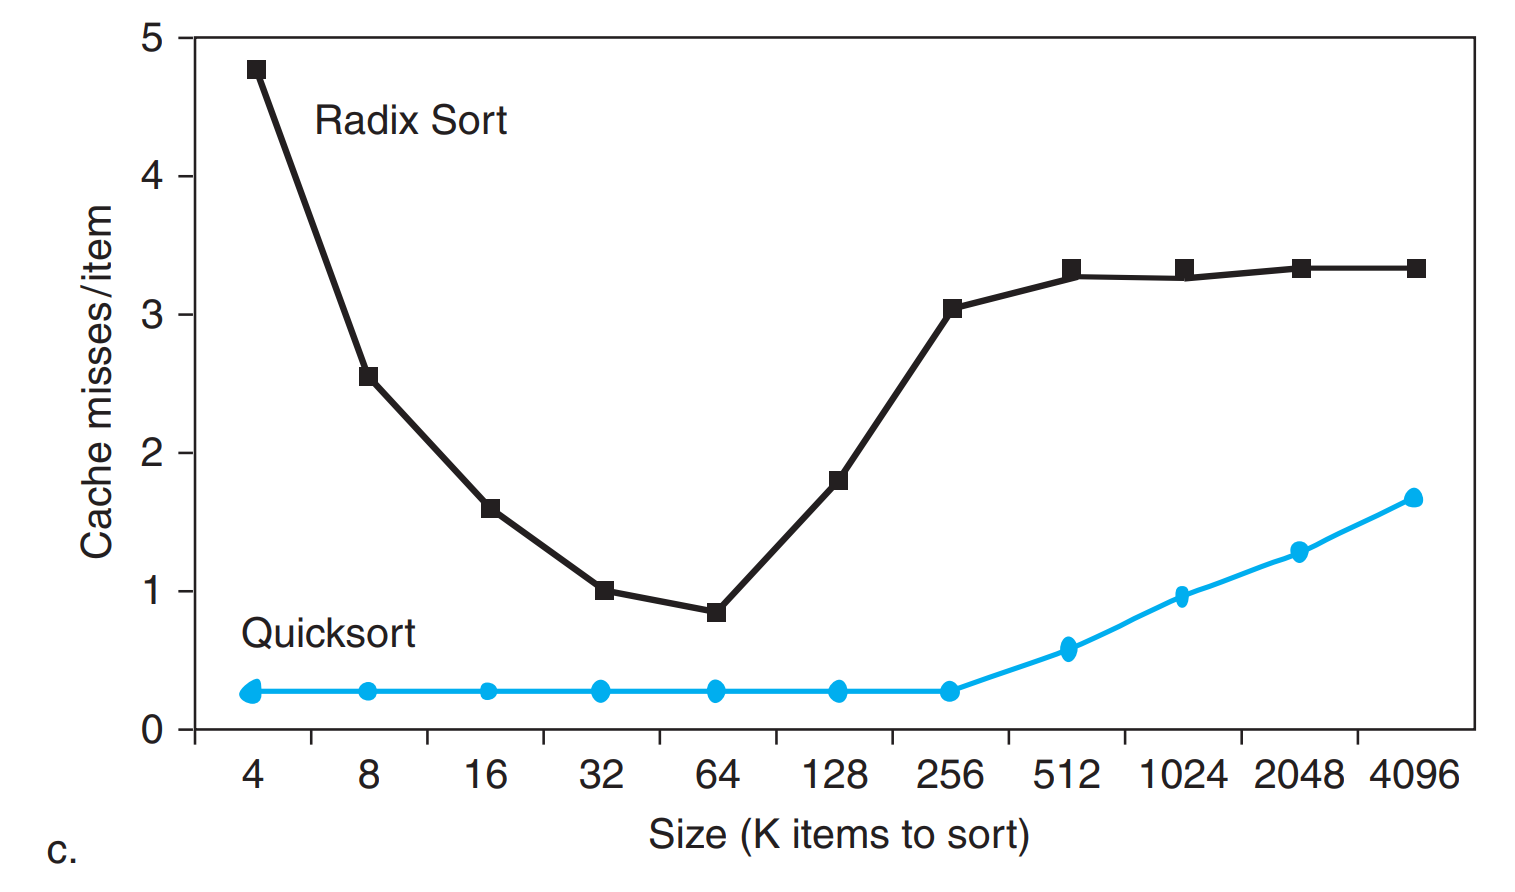
\includegraphics[scale=0.3]{{pic/quick3.png}}
    \caption{Comparing Quicksort and Radix Sort by (a) instructions executed per item sorted (b) time per item sorted, and (c) cache misses per item sorted. This data is from a paper by LaMarca and Ladner [1996]. Due to such results, new versions of Radix Sort have been invented that take memory hierarchy into account, to regain its algorithmic advantages. Th e basic idea of cache optimizations is to use all the data in a block repeatedly before it is replaced on a miss.\cite{reference2}}
\end{figure}

\newpage
%%%%%%%%%%%%%%%%%%%%%%%%%%%%%%%%%%%%%%%%%%%%%%%%%%%%%%%%%%%%%%%%%%%%%%%%%%%%



\section{개선}

\subsection{재귀함수 제거}

재귀 함수를 사용했을때에 loop문과 비교했을때 나타나는 문제점은 다음이 있다. 

\begin{itemize}
    \item 함수스택의 오버헤드
    \item 스택 오버플로우 위험성
    \item 메모리 부과    
\end{itemize}

그러나 quick sort의 반복문 사용은 복잡하며 코드가독성이 떨어진다.

\subsection{hybrid sort}

\subsubsection{Introsort}
Quicksort는 입력값에 대한 의존도가 크기에 일정 깊이로 들어같을 경우 이 밑을 heapsort로 처리하게 한다. heapsort는 Quicksort와 같은 시간복잡도가 $O(n \log n)$이지만 최선,최악에대해서 비교적 평균적인 수행시간을 보장한다. 일반적으로 한계 깊이를 $2\log_2 n$으로 설정하고있다.

\subsubsection{Quick insertion sort}
삽입 정렬(insertion sort)의 시간 복잡도는 $O(n^2)$이지만 베스트 케이스의 경우(완전히 정렬되있는경우) $O(n)$이다.(탐색만하고 넘어가기때문) 또한 작은 n에 대해서는 상대적으로 삽입정렬이 더 빠르게 되어 퀵소트 분할중 분할크기가 일정 n이하가 되면 삽입정렬으로 처리해 실제 quick sort를 사용했을때보다 시간적인 이득을 볼 수 있다. 또한 중복처리에 대해서 처리가 매우 빠르기 때문에 이에의한 성능향상도 생각해 볼 수 있다.
이 n은 일반적으로 10이며 이 값보다 작을때 선택정렬을 수행하도록한다. 

다음은 선택정렬을 수행하는 $n$에따른 수행시간이다. 여기서 테스트 케이스의 $N =10000$ 이다.

\begin{figure}[h!]
    \centering
    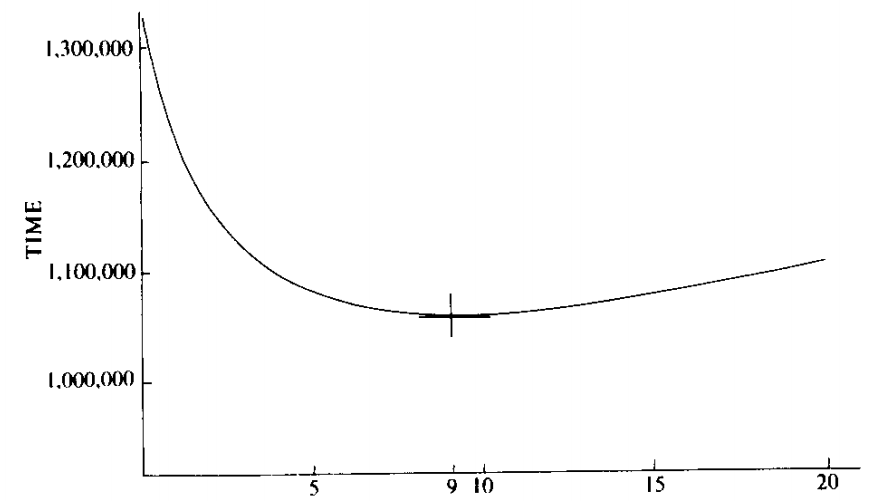
\includegraphics[scale=0.5]{{pic/q6.png}}
    \caption{삽입정렬 수행의 분할크기 n에 따른 퀵정렬 수행시간\cite{reference3}}
\end{figure}

\begin{lstlisting}[style = CStyle]
INSERTION_SORT(A)
    for j = 2 to A.length
        key = A[j]
        i = j - 1
        while i > 0 and A[i] > key
            A[i+1] = A[i]
            i = i-1
        A[i+1] = key
\end{lstlisting}

\subsection{중복값 처리}
네덜란드 국기 문제(Dutch national flag problem)로 다익스트라가 처음 제시한 이 문제는 quick sort의 중복값 입력에 대한 처리 문제를 다룬다. 배열에 같은 값으로만 들어왔을때를 생각해보자. 같은 값이 들어왔음에도 재귀는 $lg n$까지 깊이 들어간다. 이를 해결하기 위해 분할을 세 가지로한다.이를 3 way partitioning이라고한다. 기존의 왼쪽 오른쪽은 기존의 피봇값보다 \textbf{크고 작은}값이 들어가고 가운데에는 피봇과 같은 값을 모은다 그런후에 재귀의 범위를 왼쪽 오른쪽으로만 한다. 다음은 Dijstra가 제안한 해답이다. 코드는 c++로 작성되어 있다.
%\url{http://www.cs.princeton.edu/courses/archive/fall12/cos226/lectures/23Quicksort-2x2.pdf}
%https://www.cs.princeton.edu/~rs/talks/QuicksortIsOptimal.pdf

\begin{figure}[h!]
    \centering
    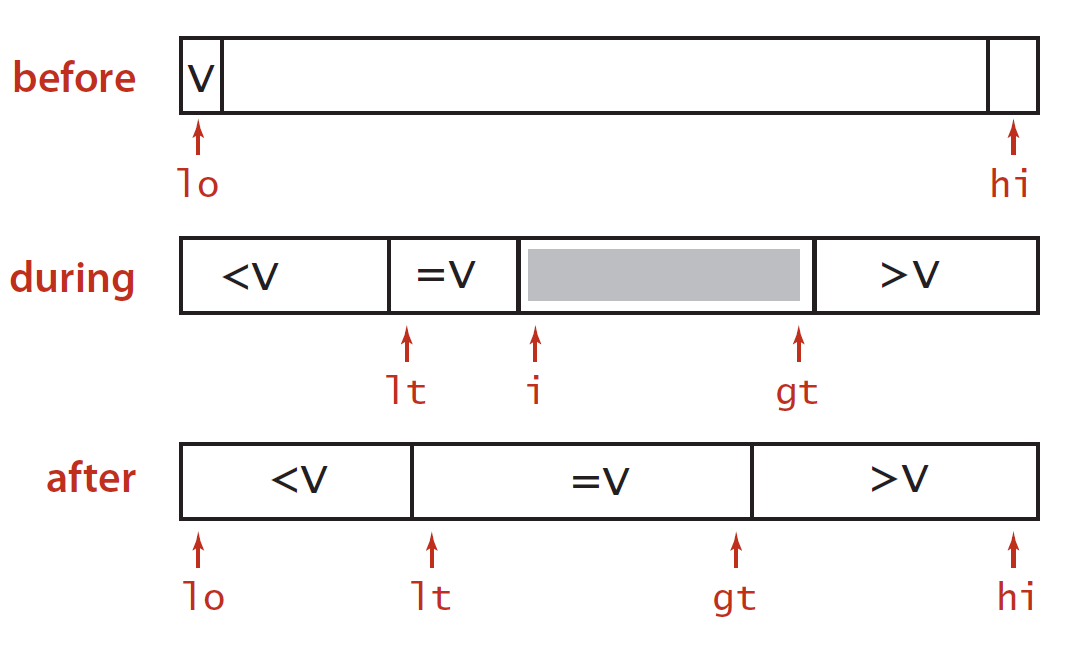
\includegraphics[scale=0.4]{{pic/q10.png}}
    \caption{3-way-partitioning 작동 방식 \cite{reference4}}
\end{figure}

\newpage


\begin{lstlisting}[style = CStyle]
void Quick3way(int a[], int lo, int hi)
{
    if (hi <= lo)
        return;
    int lt = lo, i = lo + 1, gt = hi;
    int v = a[lo];
    while (i <= gt)
    {
        if (a[i] < v)
        {
            std::swap(a[lt], a[i]);
            lt++, i++;
        }
        else if (a[i] > v)
        {
            std::swap(a[gt], a[i]);
            gt--;
        }
        else //a[i]==v
        {
            i++;
        }
    }
    Quick3way(a, lo, lt - 1);
    Quick3way(a, gt + 1, hi);
}
\end{lstlisting}

%\newpage

다음은 J. Bentley과 D. McIlroy 제안한 좀더 빠른 의사코드이다.

\begin{figure}[h!]
    \centering
    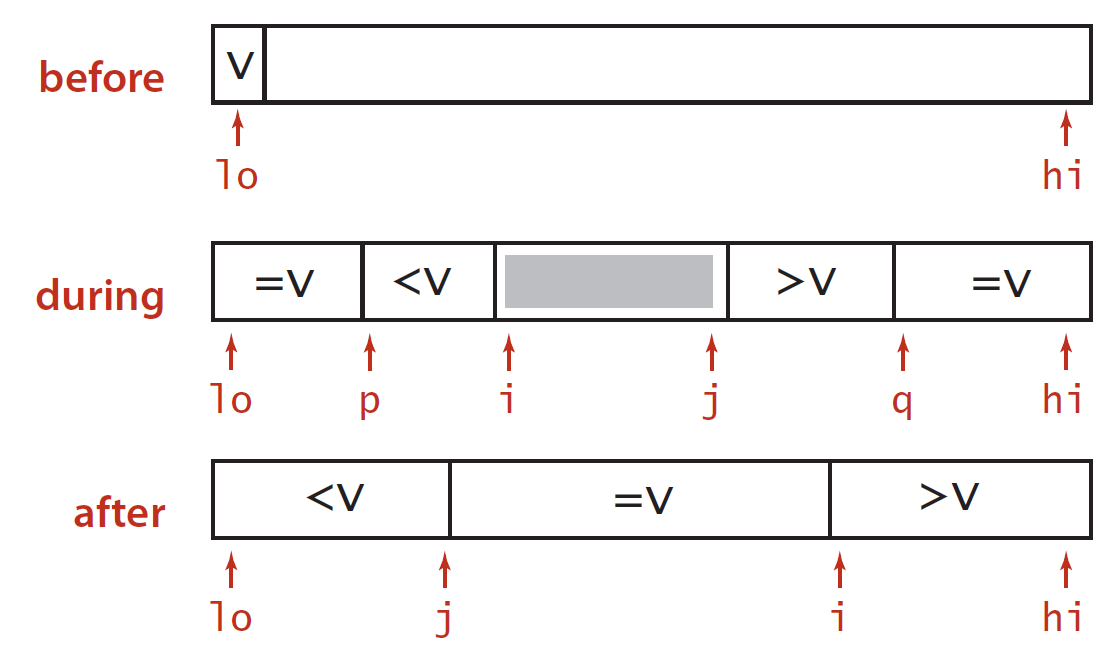
\includegraphics[scale=0.4]{{pic/q11.png}}
    \caption{Fast 3-way partitioning 작동 방식 \cite{reference4}}
\end{figure}

\begin{lstlisting}[style = CStyle]
    void quicksort(Item a[], int l, int r) 
    { 
        int i = l-1, j = r, p = l-1, q = r; Item v = a[r];
        if (r <= l) return;
        for (;;)
        {
            while (a[++i] < v) ;
            while (v < a[--j]) 
                if (j == l) break;
            if (i >= j) 
                break;
            exch(a[i], a[j]);
            if (a[i] == v) 
            {
                p++; 
                exch(a[p], a[i]); 
            }
            if (v == a[j]) 
            { 
                q--; 
                exch(a[j], a[q]); 
            }
        }
        exch(a[i], a[r]); 
        j = i-1; 
        i = i+1;
        for (k = l; k < p; k++, j--) 
            exch(a[k], a[j]);
        for (k = r-1; k > q; k--, i++) 
            exch(a[i], a[k]);
        quicksort(a, l, j);
        quicksort(a, i, r);
    }
    \end{lstlisting}

    

%http://penguin.ewu.edu/class/class/cscd300/Topic/AdvSorting/Sedgewick.pdf
\subsection{median of three}
Sedgewick이 제안했다. 위의 의사코드는 pivot값으로 맨끝의 값을 설정한다. 이는 역순정렬에 의한 최악의 케이스를 생성하기 때문에 이를 입력 p,r의 중점을 피봇값으로 설정하는것만으로도 상수시간에 개선가능하며, 이에 대한 응용으로 값을 랜덤으로 세개 뽑은후 중간값으로 하는 방법도 있다.

\subsection{Parallelization}
리커젼으로 나눠지는 두분할은 각각의 메모리 침범을 하지않는것이 명확하기 때문에 쓰레드 분할로 처리해도 문제가 없다. 이때의 가장 이상적인 수행시간은 트리 깊이인 $O(\lg n)$이다. 성능에 대해서는 병렬화의 고질적인 문제들도 복합적으로 고려해야한다.

 
and ...
멀티피봇에 대한 논의도 있으나 생략한다\footnote{다음이 좋은 참고 자료가 될것이다.\href{https://arxiv.org/abs/1905.00118}{Yukun Yao.(2019) A Detailed Analysis of Quicksort Algorithms with Experimental Mathematics} }. quicksort에 대한 연구는(특히 pivot설정) 매우 많이 진행되었고 진행되고있다.\footnote{원래 첫 제목은 All about Quicksort였으나 Quicksort에 대한 방대한 연구를 담아내기엔 상상이상으로 엄청난 논문이 줄을 이었다.}



\section{성능 테스트}

환경

\begin{itemize}
	\item msvc 14.2
	\item x86 Release모드
	\item C++
	\item Intel i7 7700
	\item RAM 16 GB
\end{itemize}


\newpage
\subsection{ HOARE VS LOMUTO }


\begin{table}[h!]
	\centering
	\begin{tabular}{|c|c|c|}
		\hline\hline
		횟수 & Hoare's partition & lomuto's partition \\ \hline
		1회 & 0.012 & 0.015 \\ \hline
		2회 & 0.029 & 0.031 \\ \hline
		3회 & 0.033 & 0.036 \\ \hline
		4회 & 0.02 & 0.021 \\ \hline
		5회 & 0.031 & 0.036 \\ \hline
		6회 & 0.009 & 0.012 \\ \hline
		7회 & 0.021 & 0.023 \\ \hline
		8회 & 0.031 & 0.034 \\ \hline
		9회 & 0.017 & 0.018 \\ \hline
		10회 & 0.019 & 0.02 \\ \hline
		\hline\hline
	\end{tabular}
	\caption{n = 10000000 랜덤 순열 partition 수행비교}
\end{table}

\begin{table}[h!]
	\centering
	\begin{tabular}{|c|c|c|}
		\hline\hline
		횟수 & Hoare's quick sort & lomuto's quick sort \\ \hline
		1회 & 0.719 & 0.759 \\ \hline
		2회 & 0.704 & 0.77 \\ \hline
		3회 & 0.712 & 0.764 \\ \hline
		4회 & 0.69 & 0.761 \\ \hline
		5회 & 0.698 & 0.758 \\ \hline
		6회 & 0.696 & 0.759 \\ \hline
		7회 & 0.696 & 0.769 \\ \hline
		8회 & 0.692 & 0.761 \\ \hline
		9회 & 0.697 & 0.765 \\ \hline
		10회 & 0.695 & 0.755 \\ \hline
		\hline\hline
	\end{tabular}
	\caption{n = 10000000 랜덤 순열 quicksort 수행비교}
\end{table}


\begin{table}[h!]
	\centering
	\begin{tabular}{|c|c|c|}
		\hline\hline
		횟수 & Hoare's quick sort & lomuto's quick sort \\ \hline
		1회 & 0.025 & 0.044 \\ \hline
		2회 & 0.013 & 0.04 \\ \hline
		3회 & 0.013 & 0.038 \\ \hline
		4회 & 0.014 & 0.041 \\ \hline
		5회 & 0.014 & 0.042 \\ \hline
		6회 & 0.013 & 0.044 \\ \hline
		7회 & 0.015 & 0.044 \\ \hline
		8회 & 0.014 & 0.041 \\ \hline
		9회 & 0.014 & 0.041 \\ \hline
		10회 & 0.016 & 0.042 \\ \hline
		\hline\hline
	\end{tabular}
	\caption{n = 10000 역정렬된 순열}
\end{table}


\begin{table}[h!]
	\centering
	\begin{tabular}{|c|c|c|}
		\hline\hline
		횟수 & Hoare's quick sort & lomuto's quick sort \\ \hline
		1회 & 0.023 & 0.035 \\ \hline
		2회 & 0.015 & 0.032 \\ \hline
		3회 & 0.019 & 0.037 \\ \hline
		4회 & 0.017 & 0.033 \\ \hline
		5회 & 0.012 & 0.031 \\ \hline
		6회 & 0.015 & 0.036 \\ \hline
		7회 & 0.016 & 0.036 \\ \hline
		8회 & 0.014 & 0.035 \\ \hline
		9회 & 0.015 & 0.034 \\ \hline
		10회 & 0.02 & 0.036 \\ \hline
		\hline\hline
	\end{tabular}
	\caption{n = 10000 정렬된 순열}
\end{table}

앞서 살펴본 평균적인 시간복잡도와는 다르게 partition의 실제 차이가 세배가 나지않았다.

\subsection{개선 성능 테스트}

\begin{itemize}
	\item PARALLELIZATION
	\item insertion sort 삽입
	\item 3way partition
\end{itemize}
insertion sort와 PARALLELIZATION의 파티션 분할에선 lomuto's partition을 사용했다.

\begin{lstlisting}[style = CStyle]
    
\end{lstlisting}


\begin{table}[h!]
	\centering
	\begin{tabular}{|c|c|c|}
		\hline\hline
		횟수 & PARALLELIZATION quick sort & quick sort + insertion sort(n<=10)\\ \hline
		1회 & 0.511 & 0.717 \\ \hline
		2회 & 0.605 & 0.714 \\ \hline
		3회 & 0.541 & 0.715 \\ \hline
		4회 & 0.456 & 0.711 \\ \hline
		5회 & 0.727 & 0.715 \\ \hline
		6회 & 0.771 & 0.719 \\ \hline
		7회 & 0.744 & 0.705 \\ \hline
		8회 & 0.643 & 0.711 \\ \hline
		9회 & 0.649 & 0.715 \\ \hline
		10회 & 0.721 & 0.712 \\ \hline
		\hline\hline
	\end{tabular}
	\caption{n = 10000000 랜덤한 임의 순열}
\end{table}


\begin{table}[h!]
	\centering
	\begin{tabular}{|c|c|c|}
		\hline\hline
		횟수 & lumoto's quick sort & Dijkstra's\\ \hline
		1회 & 0.778 & 0.772 \\ \hline
		2회 & 0.774 & 0.778 \\ \hline
		3회 & 0.759 & 0.777 \\ \hline
		4회 & 0.774 & 0.77 \\ \hline
		5회 & 0.761 & 0.766 \\ \hline
		6회 & 0.773 & 0.778 \\ \hline
		7회 & 0.772 & 0.782 \\ \hline
		8회 & 0.767 & 0.774 \\ \hline
		9회 & 0.777 & 0.784 \\ \hline
		10회 & 0.767 & 0.781 \\ \hline
		\hline\hline
	\end{tabular}
	\caption{n = 10000000 랜덤한 비중복 임의 순열}
\end{table}




\begin{table}[h!]
	\centering
	\begin{tabular}{|c|c|c|}
		\hline\hline
		횟수 & lumoto's quick sort &  Dijkstra's  \\ \hline
		1회 & 0.41 & 0.033 \\ \hline
		2회 & 0.39 & 0.038 \\ \hline
		3회 & 0.366 & 0.032 \\ \hline
		4회 & 0.367 & 0.03 \\ \hline
		5회 & 0.36 & 0.032 \\ \hline
		6회 & 0.357 & 0.032 \\ \hline
		7회 & 0.361 & 0.031 \\ \hline
		8회 & 0.358 & 0.032 \\ \hline
		9회 & 0.356 & 0.031 \\ \hline
		10회 & 0.365 & 0.032 \\ \hline
		\hline\hline
	\end{tabular}
	\caption{n = 10000000   $0 \sim 1000$ 범위의 중복포함한 랜덤 순열}
\end{table}



\begin{table}[h!]
	\centering
	\begin{tabular}{|c|c|c|}
		\hline\hline
		횟수 & Dijkstra's &  \protect\text{J. Bentley  D. McIlroy}    \\ \hline
		1회 & 0.036 & 0.032 \\ \hline
		2회 & 0.037 & 0.034 \\ \hline
		3회 & 0.036 & 0.031 \\ \hline
		4회 & 0.038 & 0.036 \\ \hline
		5회 & 0.04 & 0.035 \\ \hline
		6회 & 0.036 & 0.034 \\ \hline
		7회 & 0.043 & 0.031 \\ \hline
		8회 & 0.036 & 0.033 \\ \hline
		9회 & 0.038 & 0.036 \\ \hline
		10회 & 0.036 & 0.031 \\ \hline
		\hline\hline
	\end{tabular}
	\caption{n = 10000000  $0 \sim 1000$ 범위의 중복포함한 랜덤 순열}
\end{table}

\newpage

\subsection{ std::sort 성능테스트 VS J. Bentley  D. McIlroy}
std::sort는 J. Bentley  D. McIlroy의 3 way partition과 수행시간이 상당히 유사하다.
3 way partition에 inertion sort를 삽입했었는데 오버헤드 때문에 전체 수행시간이 오히려 안좋아졌다.


\begin{table}[h!]
	\centering
	\begin{tabular}{|c|c|c|c|}
		\hline\hline
		횟수 & 비중복 임의 순열 & $0 \sim 1000$ 범위의 중복을 포함한 랜덤 순열 & 모든값이 0 \\ \hline
		1회 & 0.964 & 0.38 & 0.007 \\ \hline
		2회 & 0.927 & 0.374 & 0.007 \\ \hline
		3회 & 0.959 & 0.373 & 0.007 \\ \hline
		4회 & 0.95 & 0.386 & 0.006 \\ \hline
		5회 & 0.946 & 0.381 & 0.006 \\ \hline
		6회 & 0.947 & 0.383 & 0.006 \\ \hline
		7회 & 0.947 & 0.392 & 0.006 \\ \hline
		8회 & 0.929 & 0.383 & 0.006 \\ \hline
		9회 & 0.932 & 0.385 & 0.006 \\ \hline
		10회 & 0.957 & 0.383 & 0.007 \\ \hline
		\hline\hline
	\end{tabular}
	\caption{n = 10000000 std::sort의 성능 분석}
\end{table}

\begin{table}[h!]
	\centering
	\begin{tabular}{|c|c|c|c|}
		\hline\hline
		횟수 & 비중복 임의 순열 & $0 \sim 1000$ 범위의 중복을 포함한 랜덤 순열 & 모든값이 0 \\ \hline
		1회 & 0.985 & 0.337 & 0.008 \\ \hline
		2회 & 1.011 & 0.332 & 0.008 \\ \hline
		3회 & 0.979 & 0.338 & 0.008 \\ \hline
		4회 & 0.956 & 0.336 & 0.008 \\ \hline
		5회 & 1.019 & 0.338 & 0.007 \\ \hline
		6회 & 0.974 & 0.333 & 0.007 \\ \hline
		7회 & 0.979 & 0.341 & 0.008 \\ \hline
		8회 & 0.973 & 0.341 & 0.009 \\ \hline
		9회 & 0.98 & 0.326 & 0.009 \\ \hline
		10회 & 0.98 & 0.332 & 0.008 \\ \hline
		\hline\hline
	\end{tabular}
	\caption{n = 10000000  J. Bentley  D. McIlroy의 3 way partition의 성능 분석}
\end{table}


\begin{lstlisting}[style = CStyle]
    
\end{lstlisting}




\listoffigures

\listoftables

\newpage
% https://www.overleaf.com/learn/latex/Sections_and_chapters
\addcontentsline{toc}{section}{참고 자료}
\section*{참고 자료}
\url{https://en.wikipedia.org/wiki/Quicksort} \\
\url{https://cs.stackexchange.com/questions/11458/ quicksort-partitioning-hoare-vs-lomuto} \\
\url{https://www.acmicpc.net/blog/view/58} \\
\url{https://www.youtube.com/watch?v=hq4dpyuX4Uw&list=PL52K_8WQO5oUuH06MLOrah4h05TZ4n38l&index=11} \\
\url{https://en.wikipedia.org/wiki/Recursion_(computer_science)} \\
% recursion
\url{https://algs4.tistory.com/45} \\
% h vs l testing
\url{https://arxiv.org/pdf/1905.00118.pdf} \\
\url{http://rohitja.in/lomuto-hoare-partitioning.html} \\


\url{https://www.cs.princeton.edu/~rs/talks/QuicksortIsOptimal.pdf}
\url{https://en.wikipedia.org/wiki/Dutch_national_flag_problem}\\
% 3 way partition
\url{https://en.wikipedia.org/wiki/Introsort}\\
%introsort
\url{https://www.geeksforgeeks.org/internal-details-of-stdsort-in-c/}
%std::sort simple code
\url{https://stackoverflow.com/questions/44441876/quick-sort-using-stack-in-c}
%quicksort with stack 

\url{http://fpl.cs.depaul.edu/jriely/ds1/extras/lectures/23Quicksort.pdf}

\begin{thebibliography}{}
    \bibitem{reference1}
    Thomas H. Cormen, Charles E. Leiserson, Ronald L. Rivest, and Clifford Stein. Introduction to Algorithms, Second Edition. MIT Press and McGraw-Hill, 2001. ISBN 0-262-03293-7.
    
    \bibitem{reference2}
    Patterson, David A./ Hennessy, John L. Computer Organization and Design, Fourth Edition: The Hardware/Software Interface (The Morgan Kaufmann Series in Computer Architecture and Design). 2014. ISBN-13 9788994961897, ISBN-10 8994961895

    \bibitem{reference3}
    Sedgewick, R. (1978). "Implementing Quicksort programs". Comm. ACM. 21 (10): 847–857. doi:10.1145/359619.359631.

    \bibitem{reference4}
    Robert Sedgewick, Kevin Wayne Algorithms, 4th Edition, 2001 ISBN-13: 978-0321573513

\end{thebibliography}
\end{document}

% testing
% std::sort